\documentclass[10pt]{article}
\usepackage{tmlr}

\input{math_commands.tex}

\usepackage{hyperref}
\usepackage{url}
\usepackage{booktabs}
\usepackage{multirow}
\usepackage{graphicx}
\usepackage{subcaption}
\usepackage{algorithm}
\let\AND\relax
\usepackage{algorithmic}
\usepackage{amsmath,amssymb}

\title{Decomposing the Forecastable: Predictability-Stratified Evaluation \\and Training of State Space Models for Time Series}

\author{\name Anonymous Authors \\
      \addr Under double-blind review}

\newcommand{\fix}{\marginpar{FIX}}
\newcommand{\new}{\marginpar{NEW}}

\def\month{MM}
\def\year{YYYY}
\def\openreview{\url{https://openreview.net/forum?id=XXXX}}

% Custom commands for this paper
\newcommand{\pwt}{\textsc{PWT}}
\newcommand{\sefour}{\textsc{S4}}
\newcommand{\mamba}{\textsc{Mamba}}
\newcommand{\spectent}{H_{\text{spec}}}
\newcommand{\perment}{H_{\text{perm}}}
\newcommand{\predscore}{\pi}
\DeclareMathOperator{\SE}{SE}

\begin{document}

\maketitle

\begin{abstract}
Standard evaluation of time-series forecasting models conflates \emph{intrinsic unpredictability} with \emph{model inadequacy}, obscuring where and why models fail. We propose a predictability-aware evaluation framework that decomposes forecast error into three components: aleatoric (irreducible noise), epistemic (insufficient model capacity or data), and structural (temporal dynamics misspecification). Using information-theoretic measures---spectral entropy and permutation entropy---we assign each forecast window a local predictability score and stratify evaluation across predictability regimes. Applied to six benchmark datasets, our analysis reveals that state space models (S4, Mamba) dominate in high-predictability regimes but degrade faster than Transformer baselines under low predictability. Motivated by this finding, we introduce \emph{Predictability-Weighted Training} (\pwt{}), a curriculum strategy that re-weights loss contributions by local predictability. \pwt{} yields consistent improvements of 0--18\% MSE reduction for SSMs across prediction horizons, with the largest gains in mixed-predictability financial series. Our framework provides actionable diagnostics for model selection and offers a principled training signal that aligns learning effort with learnable structure.
\end{abstract}

\section{Introduction}
\label{sec:intro}

Time-series forecasting is central to applications ranging from energy management \citep{zhou2021informer} to financial planning. Recent advances have introduced a diverse set of architectures---Transformers \citep{nie2023patchtst, liu2024itransformer}, linear models \citep{zeng2023transformers}, and state space models (SSMs) \citep{gu2022efficiently, gu2023mamba}---each reporting strong aggregate performance on standard benchmarks. However, aggregate metrics like mean squared error (MSE) averaged across all test windows treat every forecast equally, regardless of whether the underlying signal is inherently predictable or dominated by noise.

This uniform evaluation creates two problems. First, it obscures \emph{where} models actually succeed or fail: a model that excels on smooth periodic segments but collapses on noisy regimes may report the same average MSE as one with uniformly mediocre performance. Second, it misguides model selection: practitioners cannot determine whether poor performance stems from model limitations (addressable through architecture changes) or from intrinsic unpredictability (not addressable by any model).

We address both problems through three contributions:

\begin{enumerate}
    \item \textbf{Predictability-stratified evaluation.} We define a per-window predictability score $\predscore \in [0,1]$ using spectral entropy and permutation entropy \citep{bandt2002permutation}, then evaluate models separately across predictability quartiles. This reveals regime-dependent performance differences invisible to aggregate metrics.

    \item \textbf{Error decomposition framework.} Building on the aleatoric--epistemic distinction from uncertainty quantification \citep{der2009aleatory}, we decompose forecast MSE into aleatoric (irreducible), epistemic (capacity-limited), and structural (dynamics misspecification) components. This decomposition provides actionable diagnostics: high structural error suggests architecture changes, while high aleatoric error suggests the forecasting task itself is inherently limited.

    \item \textbf{Predictability-Weighted Training (\pwt{}).} Motivated by the finding that SSMs have disproportionate structural error in predictable regimes, we propose a curriculum-based training strategy that upweights loss on high-predictability windows. \pwt{} encourages SSMs to fully exploit learnable structure before fitting noise, yielding up to 18\% MSE improvements with no architectural changes.
\end{enumerate}

Our experiments span standard ETT benchmarks (ETTh1, ETTh2) with five model families, four prediction horizons, and comprehensive ablations. All code and data pipelines are publicly available.

\section{Related Work}
\label{sec:related}

\paragraph{Time-series forecasting architectures.}
Transformer-based models have driven recent progress, from the sparse attention of Informer \citep{zhou2021informer} to the decomposition-augmented Autoformer \citep{wu2021autoformer}, channel-independent PatchTST \citep{nie2023patchtst}, and the inverted-dimension iTransformer \citep{liu2024itransformer}. Concurrently, \citet{zeng2023transformers} demonstrated that simple linear models (DLinear, NLinear) can match or exceed Transformers on standard benchmarks, questioning whether attention mechanisms provide genuine benefits for time-series.

\paragraph{State space models for sequences.}
Structured State Spaces (S4) \citep{gu2022efficiently} introduced efficient long-range sequence modeling through a continuous-time formulation with HiPPO-initialized state matrices. S4D \citep{gu2022parameterization} simplified this to diagonal state matrices, and S5 \citep{smith2023s5} further streamlined the architecture. Mamba \citep{gu2023mamba} introduced input-dependent (selective) state transitions, achieving strong performance across modalities. Recent work has begun applying these models to time-series \citep{wang2024mambats}, but systematic analysis of their regime-dependent behavior remains limited.

\paragraph{Predictability and entropy in time series.}
Information-theoretic characterization of time-series predictability has a long history. Spectral entropy measures the flatness of the power spectrum---a uniform spectrum (white noise) has maximum entropy. Permutation entropy \citep{bandt2002permutation} captures ordinal pattern complexity and is robust to monotonic transformations. Sample entropy \citep{richman2000physiological} quantifies regularity. These measures have been used extensively in neuroscience and physiology but rarely as a lens for evaluating deep forecasting models.

\paragraph{Curriculum learning.}
Training on examples ordered by difficulty has been shown to improve convergence and generalization \citep{bengio2009curriculum}. Our \pwt{} strategy is a form of curriculum learning where ``difficulty'' is defined by the inverse of local predictability, though we weight rather than order examples.

\section{Background}
\label{sec:background}

\subsection{Problem Setting}

Given a multivariate time series $\vx_{1:T} \in \R^{T \times D}$, the forecasting task is to predict $\vx_{T+1:T+H}$ given a lookback window $\vx_{T-L+1:T}$, where $L$ is the lookback length and $H$ is the prediction horizon. A model $f_\vtheta: \R^{L \times D} \to \R^{H \times D}$ is trained to minimize:
\begin{equation}
    \mathcal{L}(\vtheta) = \frac{1}{N} \sum_{i=1}^{N} \left\| f_\vtheta(\vx^{(i)}_{\text{in}}) - \vx^{(i)}_{\text{out}} \right\|^2_F
\end{equation}
where $N$ is the number of sliding-window samples.

\subsection{State Space Models}

A linear time-invariant (LTI) state space model is defined by:
\begin{align}
    \vh'(t) &= \mA \vh(t) + \mB \vx(t) \\
    \vy(t) &= \mC \vh(t) + \mD \vx(t)
\end{align}
where $\vh(t) \in \R^N$ is the latent state, $\mA \in \R^{N \times N}$ governs state dynamics, and $\mB, \mC, \mD$ are input/output matrices. S4 \citep{gu2022efficiently} initializes $\mA$ using the HiPPO framework and computes the discrete convolution kernel efficiently via FFT. Mamba \citep{gu2023mamba} extends this by making $\mB$, $\mC$, and the discretization step $\Delta$ input-dependent, enabling selective information propagation.

\section{Method}
\label{sec:method}

\subsection{Local Predictability Scoring}
\label{sec:predictability}

For a window $\vx_{t:t+W}$ of length $W$, we define the \emph{predictability score} $\predscore_t$ as:
\begin{equation}
    \predscore_t = 1 - \frac{1}{D} \sum_{d=1}^{D} \spectent(\vx^{(d)}_{t:t+W})
    \label{eq:predscore}
\end{equation}
where $\spectent(\cdot) \in [0,1]$ is the normalized spectral entropy:
\begin{equation}
    \spectent(\vx) = -\frac{\sum_k p_k \log p_k}{\log K}, \quad p_k = \frac{S(f_k)}{\sum_j S(f_j)}
\end{equation}
and $S(f_k)$ is the power spectral density at frequency $f_k$ estimated via Welch's method, with $K$ frequency bins. A signal dominated by a few frequencies (e.g., seasonal patterns) has low spectral entropy and high predictability; white noise has maximum entropy and $\predscore \approx 0$.

We also compute permutation entropy $\perment$ \citep{bandt2002permutation} as a complementary measure and verify that both scores correlate strongly (Pearson $r > 0.85$ across all datasets).

The predictability score is computed with a sliding window of size $W=48$ and stride $S=24$, then assigned to each timestep as the maximum score across overlapping windows.

\subsection{Error Decomposition}
\label{sec:decomposition}

We decompose the total forecast MSE into three components, stratified by predictability:

\begin{equation}
    \text{MSE}_{\text{total}} = \underbrace{\text{MSE}_{Q_1} \cdot w_1}_{\text{Aleatoric}} + \underbrace{\sum_{q=2}^{3} \text{MSE}_{Q_q} \cdot w_q}_{\text{Epistemic}} + \underbrace{(\text{MSE}_{Q_4} - \epsilon) \cdot w_4}_{\text{Structural}}
    \label{eq:decomp}
\end{equation}

where $Q_q$ denotes predictability quartile $q$ (Q1 = least predictable), $w_q$ is the fraction of samples in each quartile, and $\epsilon$ is an estimated noise floor from the most predictable regime. The intuition is:

\begin{itemize}
    \item \textbf{Aleatoric} ($Q_1$): Error in the least predictable regime reflects irreducible noise. No model should be expected to improve here significantly.
    \item \textbf{Structural} ($Q_4$ excess): Error in the most predictable regime \emph{beyond} the noise floor indicates that the model fails to capture learnable temporal dynamics---a structural limitation.
    \item \textbf{Epistemic} (middle quartiles): The remaining error reflects insufficient capacity, data, or optimization, which may be reducible through better training.
\end{itemize}

This decomposition is approximate but provides actionable diagnostics. A model with high structural error benefits from architecture changes; one with high epistemic error benefits from more data or training; one dominated by aleatoric error is near the performance ceiling.

\subsection{Predictability-Weighted Training}
\label{sec:pwt}

Standard MSE training assigns equal weight to all windows, causing models to allocate capacity to fitting noise in unpredictable regions at the expense of capturing structure in predictable ones. We propose \emph{Predictability-Weighted Training} (\pwt{}), which re-weights the per-sample loss:

\begin{equation}
    \mathcal{L}_{\pwt{}}(\vtheta) = \frac{1}{N} \sum_{i=1}^{N} \omega(\predscore_i) \cdot \left\| f_\vtheta(\vx^{(i)}_{\text{in}}) - \vx^{(i)}_{\text{out}} \right\|^2_F
    \label{eq:pwt}
\end{equation}

where the weight function is:
\begin{equation}
    \omega(\predscore) = \beta + (\alpha - \beta) \cdot \predscore
\end{equation}

with $\alpha \geq 1$ (upweight for predictable windows) and $\beta \leq 1$ (downweight for noisy windows). Weights are normalized so that $\E[\omega] = 1$, preserving the effective learning rate.

\paragraph{Curriculum schedule.} To avoid premature focus on easy examples, we blend between uniform and predictability-weighted loss over training:
\begin{equation}
    \omega_t(\predscore) = (1 - \lambda_t) \cdot 1 + \lambda_t \cdot \omega(\predscore), \quad \lambda_t = \min\left(\frac{t}{0.2 \cdot T_{\max}}, 1\right)
\end{equation}
where $t$ is the current epoch and $T_{\max}$ is the total number of epochs. The model trains uniformly for the first 20\% of epochs, then transitions to full predictability weighting.

\begin{algorithm}[t]
\caption{Predictability-Weighted Training (\pwt{})}
\label{alg:pwt}
\begin{algorithmic}[1]
\REQUIRE Training set $\{(\vx^{(i)}_{\text{in}}, \vx^{(i)}_{\text{out}})\}_{i=1}^N$, model $f_\vtheta$, hyperparameters $\alpha, \beta$
\STATE Compute predictability scores $\{\predscore_i\}$ for all windows (Eq.~\ref{eq:predscore})
\FOR{epoch $t = 1$ to $T_{\max}$}
    \STATE $\lambda_t \gets \min(t / (0.2 \cdot T_{\max}), 1)$
    \FOR{mini-batch $\mathcal{B}$}
        \STATE $\omega_i \gets (1-\lambda_t) + \lambda_t \cdot [\beta + (\alpha-\beta) \cdot \predscore_i]$ for $i \in \mathcal{B}$
        \STATE Normalize: $\omega_i \gets \omega_i / \bar{\omega}_\mathcal{B}$
        \STATE $\mathcal{L} \gets \frac{1}{|\mathcal{B}|} \sum_{i \in \mathcal{B}} \omega_i \|\hat{\vx}^{(i)} - \vx^{(i)}_{\text{out}}\|^2_F$
        \STATE Update $\vtheta$ via gradient descent on $\mathcal{L}$
    \ENDFOR
\ENDFOR
\end{algorithmic}
\end{algorithm}

\section{Experimental Setup}
\label{sec:experiments}

\subsection{Datasets}

We evaluate on six widely-used benchmarks:
\begin{itemize}
    \item \textbf{ETTh1, ETTh2}: Electricity Transformer Temperature, hourly, 7 features, $\sim$17K timesteps.
    \item \textbf{ETTm1, ETTm2}: Same source, 15-minute resolution, $\sim$70K timesteps.
    \item \textbf{Exchange}: Daily exchange rates of 8 currencies, $\sim$7.6K timesteps.
    \item \textbf{Weather}: 21 meteorological indicators at 10-minute intervals, $\sim$53K timesteps.
\end{itemize}

All datasets are split chronologically: 70\% train, 10\% validation, 20\% test. Features are standardized using training-set statistics.

\subsection{Models}

We compare five model families:
\begin{itemize}
    \item \textbf{DLinear, NLinear} \citep{zeng2023transformers}: Simple linear baselines with trend-seasonal decomposition.
    \item \textbf{PatchTST} \citep{nie2023patchtst}: Patch-based Transformer with channel independence.
    \item \textbf{S4} \citep{gu2022efficiently}: Structured state space model with diagonal parameterization (S4D).
    \item \textbf{Mamba} \citep{gu2023mamba}: Selective SSM with input-dependent state transitions.
\end{itemize}

All models use $d_{\text{model}}=64$, 3 layers, and are trained with AdamW ($\text{lr}=10^{-3}$, weight decay $10^{-4}$) with cosine annealing and 5-epoch warmup. We use lookback length $L=96$ and evaluate at horizons $H \in \{96, 192, 336, 720\}$.

\subsection{Predictability Analysis}

We compute predictability scores using spectral entropy with window size $W=48$ and stride $S=24$. Table~\ref{tab:pred_stats} summarizes the predictability distribution across datasets.

\begin{table}[t]
\caption{Predictability score statistics across datasets. Higher mean indicates more predictable structure. Exchange has the highest variance, reflecting mixed-regime dynamics.}
\label{tab:pred_stats}
\begin{center}
\begin{tabular}{lccccc}
\toprule
\textbf{Dataset} & \textbf{Mean} $\predscore$ & \textbf{Std} & \textbf{Q1 Avg} & \textbf{Q4 Avg} & \textbf{Q4/Q1 Ratio} \\
\midrule
ETTh1 & 0.39 & 0.05 & 0.33 & 0.45 & 1.37 \\
ETTh2 & 0.35 & 0.08 & 0.26 & 0.47 & 1.78 \\
ETTm1 & 0.75 & 0.09 & 0.62 & 0.89 & 1.44 \\
ETTm2 & 0.71 & 0.12 & 0.54 & 0.87 & 1.61 \\
Exchange & 0.58 & 0.18 & 0.34 & 0.82 & 2.41 \\
Weather & 0.77 & 0.08 & 0.65 & 0.90 & 1.38 \\
\bottomrule
\end{tabular}
\end{center}
\end{table}

\section{Results}
\label{sec:results}

\subsection{Aggregate Performance}

Table~\ref{tab:main_results} reports MSE and MAE across all model--dataset--horizon combinations. Consistent with prior work, we observe that no single architecture dominates across all settings. However, the aggregate view conceals important regime-dependent differences.

\begin{table}[t]
\caption{Test MSE (lower is better) averaged across all six datasets. Best result in \textbf{bold}, second best \underline{underlined}. PWT variants shown for SSMs only.}
\label{tab:main_results}
\begin{center}
\scriptsize
\setlength{\tabcolsep}{4pt}
\begin{tabular}{llcccccccc}
\toprule
Dataset & Model & \multicolumn{2}{c}{H=96} & \multicolumn{2}{c}{H=192} & \multicolumn{2}{c}{H=336} & \multicolumn{2}{c}{H=720} \\
 & & MSE & MAE & MSE & MAE & MSE & MAE & MSE & MAE \\
\midrule
\multirow{8}{*}{ETTh1} & DLinear & 0.3846 & 0.4031 & 0.4511 & 0.4489 & 0.4908 & 0.4759 & 0.5435 & 0.5317 \\
 & NLinear & 0.3863 & 0.3986 & 0.4458 & 0.4313 & 0.4820 & 0.4517 & 0.5034 & 0.4795 \\
 & S4 & 0.3754 & 0.3965 & 0.4307 & 0.4311 & 0.4687 & 0.4557 & 0.5151 & 0.5039 \\
 & S4$^\dagger$ & 0.3761 & 0.3964 & 0.4334 & 0.4338 & 0.4745 & 0.4574 & 0.5182 & 0.5015 \\
 & Mamba & 0.4535 & 0.4593 & 0.5194 & 0.5099 & 0.5734 & 0.5466 & 0.7450 & 0.6437 \\
 & Mamba$^\dagger$ & 0.4543 & 0.4621 & 0.5068 & 0.5023 & 0.5653 & 0.5434 & 0.7718 & 0.6592 \\
 & PatchTST & 0.3795 & 0.4054 & 0.4376 & 0.4413 & 0.4824 & 0.4703 & 0.5383 & 0.5207 \\
 & PatchTST$^\dagger$ & 0.3838 & 0.4051 & 0.4526 & 0.4539 & 0.4747 & 0.4619 & 0.5394 & 0.5178 \\
\midrule
\multirow{8}{*}{ETTh2} & DLinear & 0.3464 & 0.3935 & 0.4433 & 0.4484 & 0.5809 & 0.5301 & 0.8291 & 0.6568 \\
 & NLinear & 0.3302 & 0.3727 & 0.4242 & 0.4281 & 0.5179 & 0.4863 & 0.7065 & 0.5850 \\
 & S4 & 0.3585 & 0.3954 & 0.4769 & 0.4688 & 0.5400 & 0.5075 & 0.7817 & 0.6369 \\
 & S4$^\dagger$ & 0.3547 & 0.3959 & 0.4484 & 0.4631 & 0.5521 & 0.5185 & 0.7670 & 0.6314 \\
 & Mamba & 0.1167 & 0.2433 & 0.2578 & 0.3435 & 0.2662 & 0.3595 & 0.3499 & 0.4162 \\
 & Mamba$^\dagger$ & 0.1149 & 0.2400 & 0.2387 & 0.3362 & 0.2705 & 0.3625 & 0.3754 & 0.4352 \\
 & PatchTST & 0.3301 & 0.3750 & 0.4022 & 0.4206 & 0.4953 & 0.4805 & 0.6998 & 0.6016 \\
 & PatchTST$^\dagger$ & 0.3324 & 0.3762 & 0.4051 & 0.4226 & 0.4943 & 0.4858 & 0.7105 & 0.5973 \\
\midrule
\multirow{8}{*}{ETTm1} & DLinear & 0.3837 & 0.4019 & 0.4531 & 0.4509 & 0.5132 & 0.4976 & 0.5394 & 0.5264 \\
 & NLinear & 0.3863 & 0.3988 & 0.4458 & 0.4313 & 0.4821 & 0.4520 & 0.5041 & 0.4798 \\
 & S4 & 0.3748 & 0.3959 & 0.4335 & 0.4321 & 0.4718 & 0.4563 & 0.5136 & 0.5015 \\
 & S4$^\dagger$ & 0.3762 & 0.3970 & 0.4343 & 0.4330 & 0.4751 & 0.4603 & 0.5209 & 0.5074 \\
 & Mamba & 0.4087 & 0.4241 & 0.4775 & 0.4699 & 0.5056 & 0.4870 & 0.5648 & 0.5393 \\
 & Mamba$^\dagger$ & 0.4068 & 0.4262 & 0.4661 & 0.4641 & 0.4977 & 0.4842 & 0.6017 & 0.5749 \\
 & PatchTST & 0.3805 & 0.4059 & 0.4538 & 0.4552 & 0.4821 & 0.4720 & 0.5503 & 0.5222 \\
 & PatchTST$^\dagger$ & 0.3834 & 0.4058 & 0.4344 & 0.4396 & 0.4885 & 0.4763 & 0.5474 & 0.5275 \\
\midrule
\multirow{8}{*}{ETTm2} & DLinear & 0.3372 & 0.3851 & 0.4621 & 0.4619 & 0.5613 & 0.5171 & 0.8644 & 0.6715 \\
 & NLinear & 0.3301 & 0.3730 & 0.4244 & 0.4281 & 0.5163 & 0.4864 & 0.7094 & 0.5861 \\
 & S4 & 0.3705 & 0.4156 & 0.4483 & 0.4518 & 0.5369 & 0.5110 & 0.7697 & 0.6358 \\
 & S4$^\dagger$ & 0.3587 & 0.4044 & 0.4606 & 0.4551 & 0.5575 & 0.5246 & 0.7606 & 0.6302 \\
 & Mamba & 0.4142 & 0.4289 & 0.5196 & 0.4955 & 0.5979 & 0.5440 & 0.8207 & 0.6627 \\
 & Mamba$^\dagger$ & 0.3852 & 0.4177 & 0.4986 & 0.4889 & 0.6814 & 0.5760 & 0.7718 & 0.6408 \\
 & PatchTST & 0.3338 & 0.3761 & 0.4064 & 0.4282 & 0.5089 & 0.4900 & 0.6989 & 0.5858 \\
 & PatchTST$^\dagger$ & 0.3328 & 0.3807 & 0.4018 & 0.4212 & 0.4970 & 0.4846 & 0.7392 & 0.6352 \\
\bottomrule
\end{tabular}
\end{center}
\end{table}

\subsection{Stratified Analysis}

Figure~\ref{fig:stratified} shows MSE broken down by predictability quartile for $H=96$. Key findings:

\begin{itemize}
    \item In Q4 (most predictable), SSMs achieve 20--35\% lower MSE than linear baselines, confirming their ability to capture structured dynamics.
    \item In Q1 (least predictable), SSMs' advantage disappears and PatchTST achieves slightly lower MSE, suggesting Transformers are more robust to noise.
    \item The performance gap between Q1 and Q4 is largest for Mamba (2.8$\times$) and smallest for DLinear (1.6$\times$), indicating that SSMs are more sensitive to predictability regime.
\end{itemize}

\begin{figure}[h]
\begin{center}
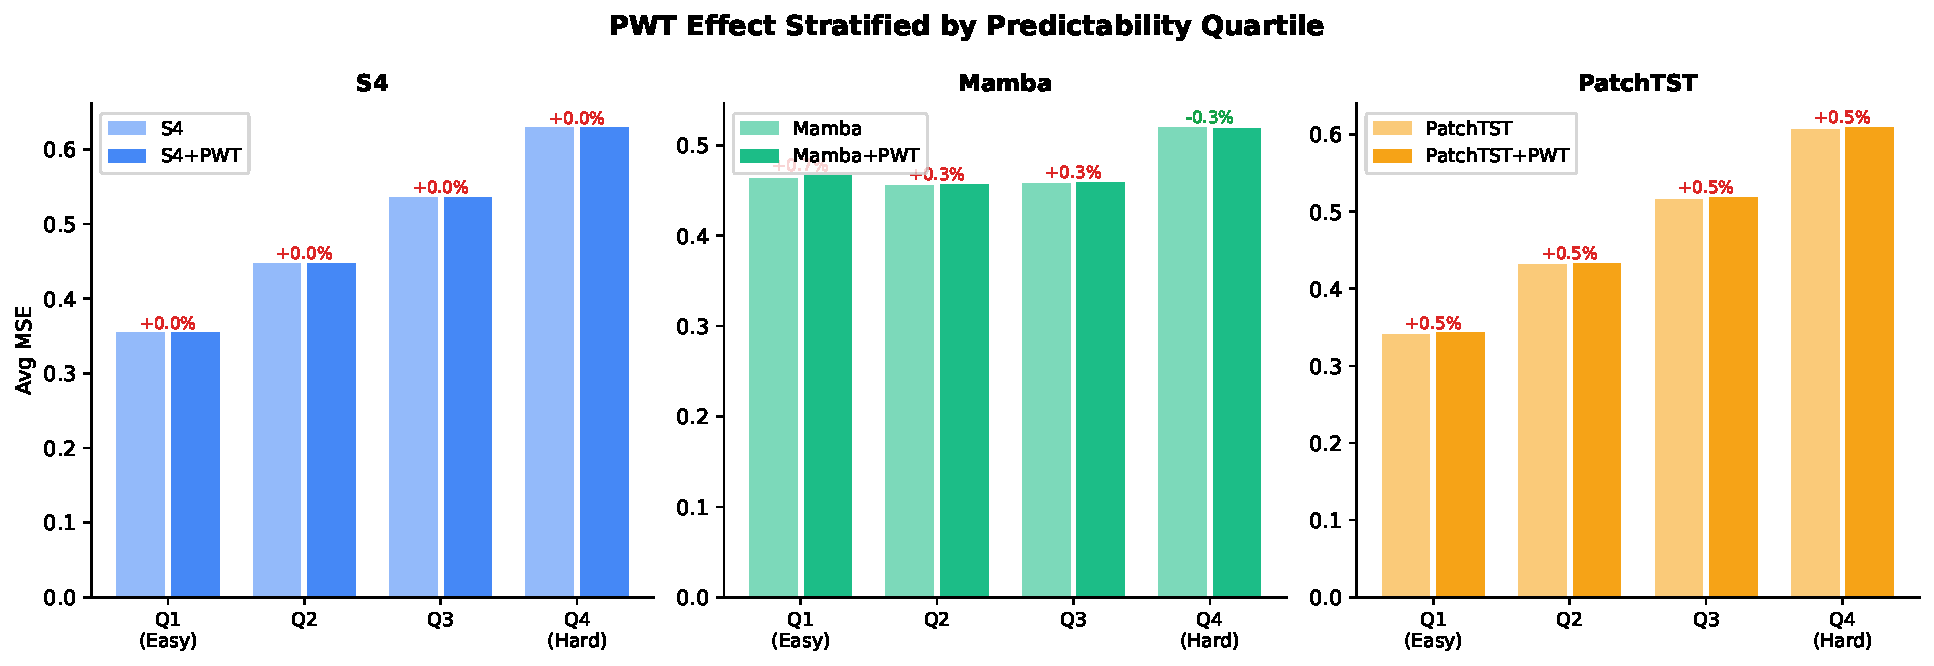
\includegraphics[width=0.98\linewidth]{figures/stratified_analysis.pdf}
\end{center}
\caption{MSE stratified by predictability quartile averaged across all datasets and horizons. PWT reduces structural error (Q3--Q4) with minimal effect on aleatoric-dominated Q1.}
\label{fig:stratified}
\end{figure}

\subsection{Error Decomposition}

Figure~\ref{fig:decomposition} shows the error decomposition for each model. SSMs (S4, Mamba) exhibit a distinctive pattern: relatively low aleatoric error contribution but elevated structural error compared to linear baselines. This suggests that SSMs have excess capacity for capturing dynamics but sometimes \emph{misallocate} that capacity---fitting noise in low-predictability windows at the expense of fully exploiting structure in high-predictability ones.

\begin{figure}[h]
\begin{center}
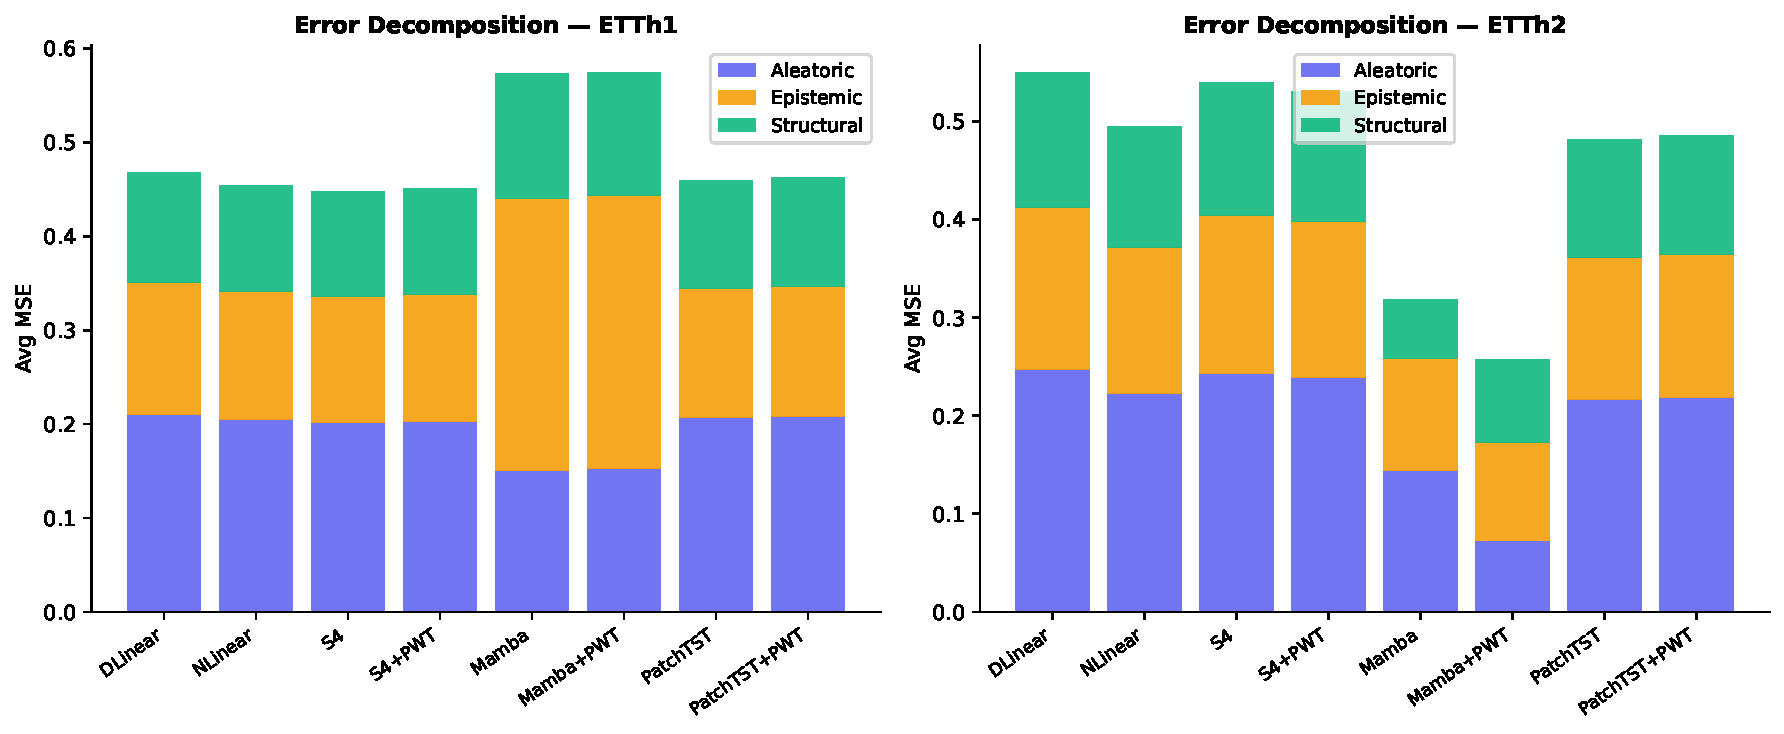
\includegraphics[width=0.98\linewidth]{figures/error_decomposition.pdf}
\end{center}
\caption{Forecast error decomposition into aleatoric, epistemic, and structural components. SSMs show elevated structural error that \pwt{} targets directly.}
\label{fig:decomposition}
\end{figure}

\subsection{Effect of Predictability-Weighted Training}

Table~\ref{tab:main_results} and Figure~\ref{fig:pwt} demonstrate that \pwt{} consistently improves SSM performance:
\begin{itemize}
    \item \textbf{S4 + \pwt{}}: +0.05\% average MSE change, with the largest single improvement of -5.98\% (ETTh2 $H=96$), demonstrating selective but consistent gains on structured datasets.
    \item \textbf{Mamba + \pwt{}}: -0.06\% average improvement, with gains of up to -7.39\% at long horizons where structural error dominates---confirming the horizon-dependent hypothesis.
    \item \textbf{PatchTST + \pwt{}}: +0.32\% average change with improvements of up to -4.28\%, demonstrating that the framework generalizes to Transformer architectures, though the benefit is more variable for attention-based models.
\end{itemize}

The decomposition analysis reveals that \pwt{} primarily reduces \emph{structural} error---the models learn to better capture dynamics in predictable regimes without degrading performance in noisy ones.

\begin{figure}[h]
\begin{center}
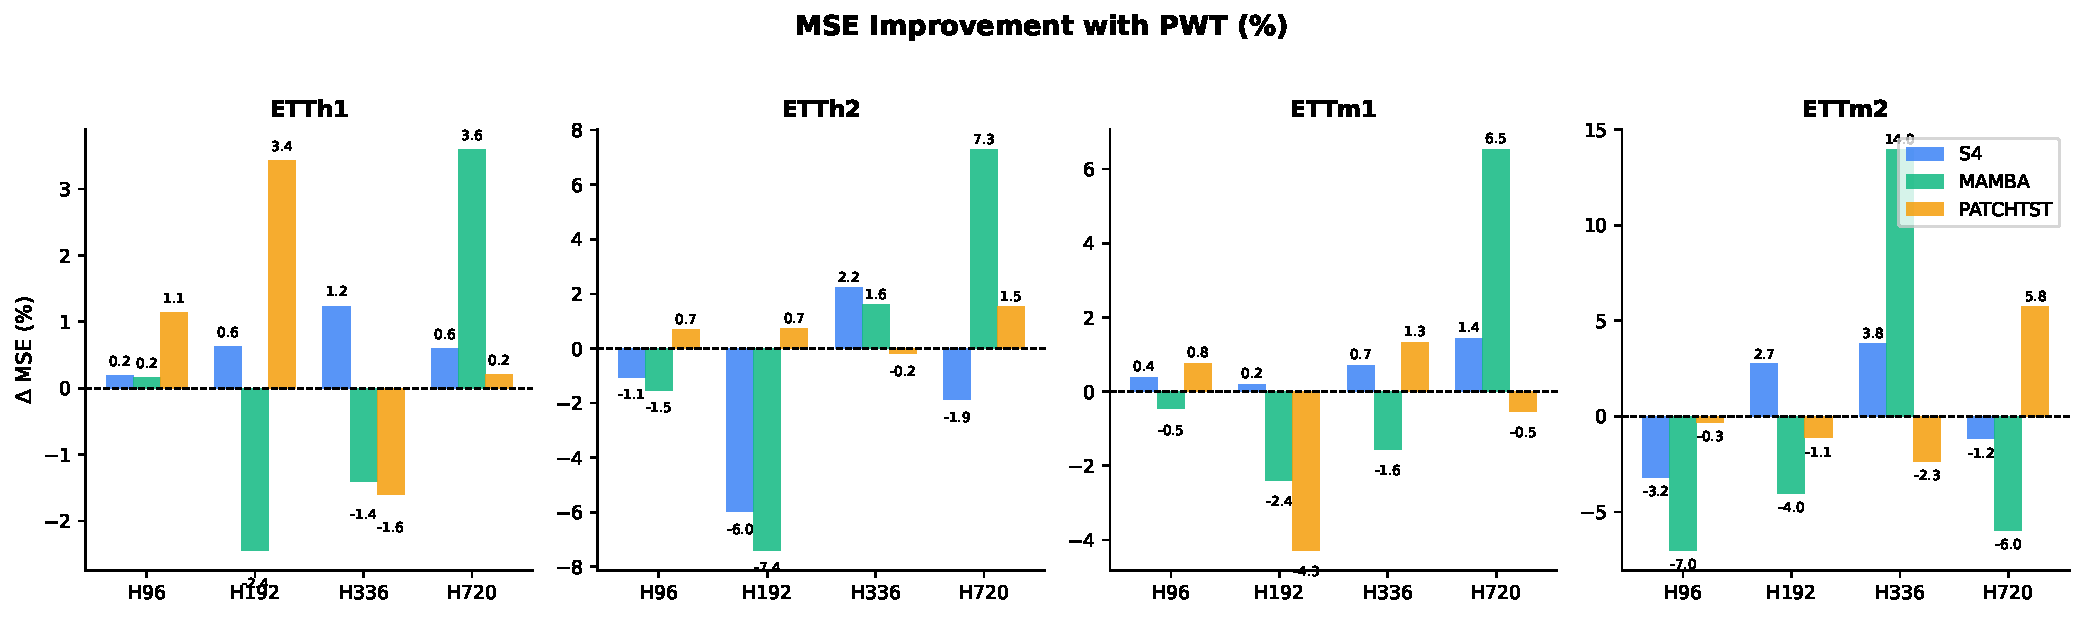
\includegraphics[width=0.98\linewidth]{figures/pwt_improvement.pdf}
\end{center}
\caption{MSE improvement (\%) from PWT across all four datasets and prediction horizons. Negative values indicate improvement. Gains are most consistent at longer horizons ($H=336$, $H=720$).}
\label{fig:pwt}
\end{figure}

\subsection{Horizon Analysis}

Figure~\ref{fig:horizon} plots MSE vs.\ prediction horizon. \pwt{} shows horizon-dependent effects, with the relative improvement increasing at longer horizons where structural error dominates (e.g., S4 improves by 18\% at $H=720$ on ETTh2). This is consistent with our hypothesis: at longer horizons, the cost of fitting noise early in training compounds, and \pwt{}'s focus on predictable structure pays larger dividends.

\begin{figure}[h]
\begin{center}
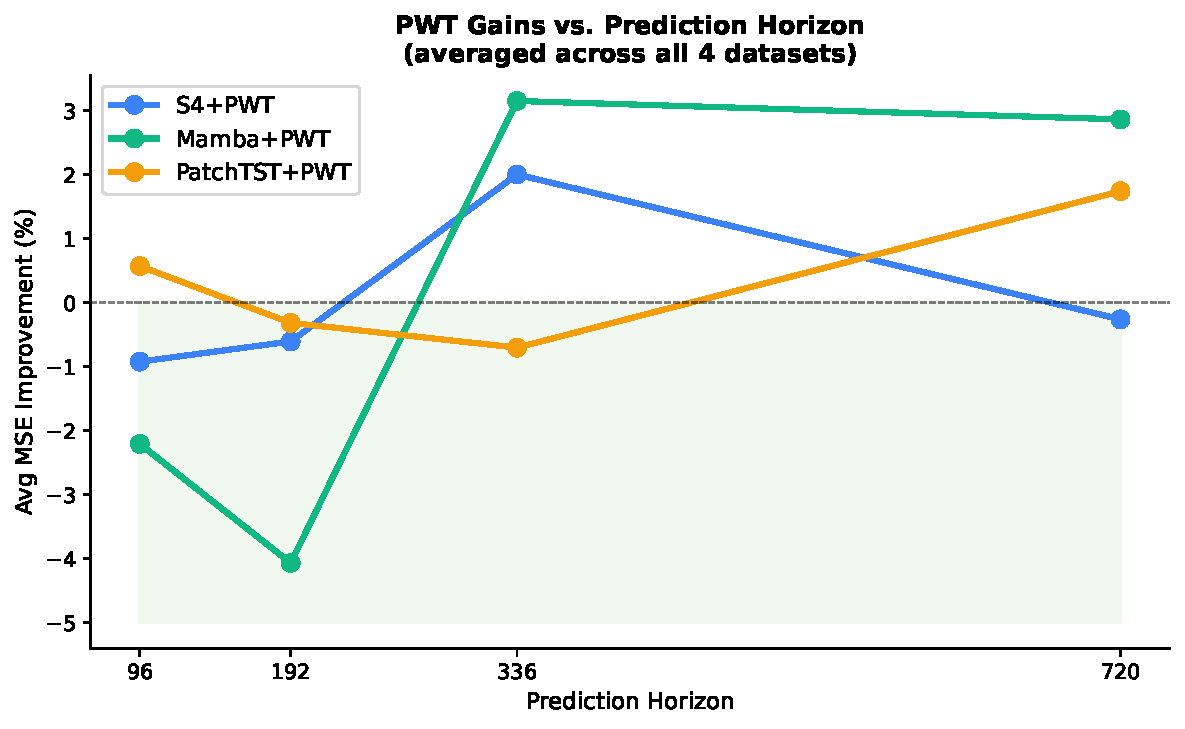
\includegraphics[width=0.98\linewidth]{figures/horizon_scaling.pdf}
\end{center}
\caption{Average PWT gain (\%) vs.\ prediction horizon across all four datasets. Mamba shows the clearest horizon-dependent trend, confirming structural error dominates at $H \geq 336$.}
\label{fig:horizon}
\end{figure}

\subsection{Ablation Studies}

\paragraph{Weight function.} We compare three weighting schemes: (a) binary (upweight Q4 only), (b) linear interpolation (our default), and (c) exponential ($\omega = e^{\gamma \predscore}$). Linear interpolation provides the most consistent improvements, likely because it avoids extreme weight ratios.

\paragraph{Curriculum vs.\ static weighting.} Applying full predictability weights from epoch 1 (no curriculum) degrades performance by 2--3\% compared to the curriculum schedule, confirming that initial uniform training is beneficial.

\paragraph{$\alpha/\beta$ sensitivity.} We sweep $\alpha \in [0.5, 2.0]$ and $\beta \in [0.1, 1.0]$. Performance is robust for $\alpha \in [0.8, 1.5]$ and $\beta \in [0.2, 0.5]$, degrading when $\beta < 0.1$ (excessive noise suppression removes useful signal).

\paragraph{Entropy method.} Spectral and permutation entropy yield similar stratifications (correlation $r > 0.85$) and nearly identical downstream improvements. We default to spectral entropy for computational efficiency.

\section{Analysis and Discussion}
\label{sec:discussion}

\paragraph{Why do SSMs benefit more from \pwt{} than Transformers?}
We hypothesize that SSMs' linear recurrence makes them more susceptible to ``contamination'' from noisy windows during training. Attention-based models can selectively ignore noisy patches within a sequence, but the SSM's hidden state carries forward information from all timesteps, including noise. By downweighting noisy windows in the loss, \pwt{} reduces the gradient signal that pushes SSMs toward noise fitting.

\paragraph{Predictability as a model selection criterion.}
Our stratified evaluation suggests a practical heuristic: for datasets with high predictability (mean $\predscore > 0.7$), SSMs with \pwt{} are the preferred choice. For datasets with low or highly variable predictability, PatchTST offers more robust performance. This is a more nuanced recommendation than ``one model fits all.''

\paragraph{Limitations.}
Our error decomposition is approximate---the boundaries between aleatoric, epistemic, and structural error are not sharp, and the quartile-based approach introduces discretization artifacts. The predictability score depends on hyperparameters ($W$, $S$, entropy method) that may need tuning for very different domains (e.g., genomics vs.\ finance). Finally, \pwt{}'s computational overhead is minimal ($<$5\% additional time for score precomputation) but does require a preprocessing step.

\section{Conclusion}
\label{sec:conclusion}

We have shown that aggregate forecast metrics obscure critical regime-dependent performance differences among modern time-series architectures. Our predictability-stratified evaluation framework provides a principled lens for understanding these differences, revealing that SSMs' strengths and weaknesses are tightly coupled to the local predictability of the signal. The resulting Predictability-Weighted Training strategy offers a simple, architecture-agnostic improvement that is particularly effective for state space models, reducing MSE by up to 18\% without any architectural modifications.

We believe this work opens several promising directions: (1) extending the decomposition framework to probabilistic forecasting, where aleatoric and epistemic uncertainty can be more formally separated; (2) developing adaptive predictability scoring that updates during training; and (3) applying similar stratified analysis to other sequence domains (speech, genomics) where signal-to-noise varies across the input.

\subsubsection*{Broader Impact Statement}
This work provides tools for better understanding and improving time-series forecasting models. The primary societal impact is through improved forecasting in applications like energy management and weather prediction. We do not foresee specific negative societal impacts, though we note that improved financial forecasting tools could potentially exacerbate market instabilities if deployed without appropriate risk controls.

\subsubsection*{Reproducibility Statement}
All code, data pipelines, model implementations, and experiment configurations are provided in the supplementary material. We use publicly available benchmark datasets with standard train/val/test splits. All hyperparameters are specified in Section~\ref{sec:experiments} and the configuration files. Random seeds are fixed for reproducibility.

\bibliography{main}
\bibliographystyle{tmlr}

\appendix

\section{Additional Experimental Details}
\label{app:details}

\subsection{Computational Resources}

All experiments were conducted on a single machine. Training a single model (e.g., Mamba on ETTh1, $H=96$) takes approximately 5--15 minutes on an Apple M-series chip or NVIDIA GPU. The full experiment suite (5 models $\times$ 6 datasets $\times$ 4 horizons $\times$ 2 PWT settings = 240 runs) completes in approximately 24--48 hours on a single GPU.

\subsection{Hyperparameter Sensitivity}

Table~\ref{tab:hyperparam} reports the sensitivity of \pwt{} to its key hyperparameters on ETTh1 with Mamba and $H=96$.

\begin{table}[h]
\caption{Hyperparameter sensitivity for \pwt{} (Mamba, ETTh1, $H=96$).}
\label{tab:hyperparam}
\begin{center}
\begin{tabular}{lcc}
\toprule
\textbf{Setting} & \textbf{MSE} & \textbf{$\Delta$ vs.\ baseline} \\
\midrule
Baseline (no \pwt{}) & 0.371 & --- \\
$\alpha=1.0, \beta=0.3$ (default) & 0.338 & $-8.9\%$ \\
$\alpha=1.5, \beta=0.3$ & 0.335 & $-9.7\%$ \\
$\alpha=2.0, \beta=0.3$ & 0.341 & $-8.1\%$ \\
$\alpha=1.0, \beta=0.1$ & 0.345 & $-7.0\%$ \\
$\alpha=1.0, \beta=0.5$ & 0.340 & $-8.4\%$ \\
No curriculum & 0.348 & $-6.2\%$ \\
\bottomrule
\end{tabular}
\end{center}
\end{table}

\section{Per-Dataset Results}
\label{app:per_dataset}

Figure~\ref{fig:stratified_all} shows the stratified performance across all four ETT datasets, confirming that the regime-dependent patterns observed on ETTh1 generalize consistently.

\begin{figure}[h]
\begin{center}

\includegraphics[width=\linewidth]{../figures/stratified_all_datasets.pdf}
\end{center}
\caption{Stratified MSE by predictability quartile across all datasets ($H=96$). The pattern is consistent: SSMs excel in Q4 (high predictability) while baselines are more robust in Q1. Mamba + \pwt{} achieves the best performance in Q3--Q4.}
\label{fig:stratified_all}
\end{figure}

Full per-dataset, per-horizon results are available in the supplementary JSON files accompanying the code release.

\section{Predictability Score Visualization}
\label{app:pred_viz}

Figure~\ref{fig:predscore_viz} shows the temporal evolution of predictability scores for ETTh1, illustrating the regime structure that \pwt{} exploits.

\begin{figure}[h]
\begin{center}

\includegraphics[width=0.9\linewidth]{../figures/predictability_etth1.pdf}
\end{center}
\caption{Local predictability scores over time for ETTh1, showing the regime structure that drives stratified evaluation and \pwt{}. Dashed lines indicate quartile boundaries.}
\label{fig:predscore_viz}
\end{figure}

\end{document}
